% This is LLNCS.DOC the documentation file of
% the LaTeX2e class from Springer-Verlag
% for Lecture Notes in Computer Science, version 2.4
\documentclass{llncs}
\usepackage{llncsdoc}
\usepackage[utf8]{inputenc}
\usepackage{listingsutf8}
\usepackage[T1]{fontenc}
\usepackage{cite}
\usepackage{graphicx}
\usepackage[ngerman]{babel}
%
\begin{document}
	\lstset{language=c++, breaklines=true, frame=single}
\markboth{Bildverarbeitung mit CUDA in C/C++}{Bildverarbeitung mit CUDA in C/C++}
\thispagestyle{empty}
%\begin{flushleft}
%\LARGE  \centering Hochschule für Technik und Wirtschaft Berlin\\ %[1cm]
%\end{flushleft}
\begin{flushleft}
\bfseries	Hochschule für Technik und Wirtschaft Berlin\\
	Fachbereich 4: Informatik Kommunikation und Wirtschaft \\
	Studiengang: Angewandte Informatik (M)\\
	Seminar: Programmierkonzepte und Algorithmen\\
	Seminarleiter: Prof. Dr. V. Brovkov und Prof. Dr. Dr. h.c. J. Sieck\\ [2.5cm]
\end{flushleft}
\vspace{45pt}
\rule{\textwidth}{1pt}
\vspace{2pt}
\begin{flushright}
\Huge
\begin{tabular}{@{}l}
Bildverarbeitung mit CUDA\\ in C/C++\\
RGBA umrechnen\\ zu luminosity grau\\[6pt]

\end{tabular}
\end{flushright}
\rule{\textwidth}{1pt}
\vfill

\begin{flushleft}
\begin{tabular}{ll}
{\bfseries Vorgelegt am 21.01.2018 durch: }\\
Florian Schwab, s0562789, s0562789@htw-berlin.de \\
Elsa Buchholz, s0544180, s0544180@htw-berlin.de \\
\end{tabular}
\end{flushleft}

%
\newpage
\tableofcontents
\newpage
%
\section{Einleitung}
%
Mit Hilfe von CUDA soll ein beliebiges Bild in verschiedene Farbkonstellationen konvertiert werden. Dabei können vier  Möglichkeiten gewählt werden; Blur, Emboss, Grün-Blau-Wechsel und luminosity grau.\\

Das Bild wird in dieser Arbeit im png-Format verarbeitet. Mit der Programmiertechnik CUDA und der Programmiersprache C/C++ wird die Bildverarbeitung auf der GPU parallelisiert, um eine hohe Rechenleistung zu realisieren.\\

Um das Bild in seinen Farbwerten verändern zu können, müssen die Pixel des Bildes, die jeweils einen RGBA-Wert speichern, in einer Matrix gespeichert werden. Danach wird mit Hilfe von CUDA ein Algorithmus verwendet, der die Pixel-Werte neu berechnet und somit eine neue RGBA-Matrix hergestellt wird. Aus dieser Matrix wird anschließend eine neue png-Datei erstellt.\\

Ein Vergleich von der Berechnung der Matrix auf der CPU anstatt auf der GPU soll zeigen, dass das sequenzielle Durchlaufen der Pixel über eine Schleife langsamer als das parallele Berechnen der Pixel auf der GPU ist. Zusätzlich wird die Programmierbibliothek OpenCV verwendet und mit CUDA verglichen. OpenCV und CUDA vollziehen beide die Berechnungen auf der GPU.\\

%
\section{Konvertierung einer PNG-Datei}
%

Eine PNG-Datei ist eine Rastergrafik, die aus Pixeln besteht. Die Gesamtheit der Pixel ergeben zusammen ein Bild, wobei jedes Pixel eine Farbe repräsentiert. Die Farbe ergibt sich aus den drei Farbkanälen rot, grün und blau und optional aus einem vierten Kanal alpha. Die Gesamtzahl der Pixel ergibt sich aus dem Produkt der Höhe und Breite des Bildes. Auf jedes Pixel des Ausgangsbilds wird eine Matrix angewandt, die die Werte der Farbkanäle enthält. Darauf werden entsprechende Algorithmen für die Konvertierung zu Emboss, Blur, luminosity grau oder für den Austausch grüner mit blauen Komponenten angewandt. Da auf jedes Pixel der gleiche Algorithmus angewandt wird, ist er für eine Parallelisierung und dementsprechend auch für CUDA geeignet.\\

Im CUDA Programmiermodel werden die CPU und die GPU für Berechnungen verwendet. Dabei wird in der CUDA Terminologie die CPU und deren Speicher als Host sowie die GPU und deren Speicher als Device bezeichnet. Der auszuführende Code wird auf dem Host ausgeführt. Vom Host aus wird der Speicher des Hosts und Devices verwaltet. Die auszuführenden Algorithmen bzw. Funktionen werden vom Kernel auf dem Device bereitgestellt. Es können ein oder mehrere Kernel aufgerufen werden, die auf dem Device mehrere Threads parallel ausführen können. Jeder Pixel repräsentiert ein Thread.\\
\newpage
Ein CUDA Programm durchläuft dementsprechend folgende Schritte:
\begin{enumerate}
	\item Zuweisung des Speicher auf dem Host und dem Device
	\item Transport der Daten vom Host auf das Device
	\item Ausführen eines oder mehrerer Kernel
	\item Transport der Ergebnisse vom Device auf den Host
\end{enumerate}

In den folgenden Abschnitten wird anhand von Code Beispielen demonstriert, wie ein CUDA Programm praktisch umgesetzt wird.\\
%Daraus entsteht eine Matrix, in der zu jedem Pixel vier Werte zugeordnet werden. Diese Matrix wird in ein Array gespeichert. Jeder Kanal kann einen Wert zwischen 0 und 255 annehmen und repräsentiert

%
\subsection{Erstellen einer RGBA Matrix aus einer PNG-Datei}
%
Die Bilddatei wird mit Hilfe der OpenCV Bibliothek geladen und gespeichert.

Das Laden und Aufbauen des Arrays für die weitere Verarbeitung erfolgt folgendermaßen:

\begin{lstlisting}
Mat raw_image = imread(argv[2], CV_LOAD_IMAGE_UNCHANGED);

// convert image/matrix to a plain 2-dim array to allow passing same input to all functions
uint32_t *image = (uint32_t *) malloc((raw_image.rows * raw_image.cols) * sizeof(uint32_t));

for (int i = 0; i < raw_image.rows; i++) {
  for (int j = 0; j < raw_image.cols; j++) {
    uint32_t raw_index = (i * raw_image.cols + j) * 4;
    uint32_t index     = (i * raw_image.cols) + j;

    // construct single integer value representing all 4 color channels
    image[index] = RGBA(raw_image.data[raw_index + 0], raw_image.data[raw_index + 1], raw_image.data[raw_index + 2], raw_image.data[raw_index + 3]);
  }
}
\end{lstlisting}
\newpage
%
\subsection{Vorbereitung der Nutzung des Devices für die Bildtransformation}
%

Mit den Funktionen CUDAMalloc() wird der nötige Speicher auf dem Device reserviert, um das Bild vom Host auf das Device kopieren zu können.

\begin{lstlisting}
size_t buffer_size = width * height * sizeof(uint32_t);
uint32_t *dev_in, *dev_out;

// Allocate memory on device
CUDA_CHECK(cudaMalloc((void **) &dev_in, buffer_size));
CUDA_CHECK(cudaMalloc((void **) &dev_out, buffer_size));
\end{lstlisting}

Auf dem Host werden weiterhin die Daten vom Speicher des Hosts in den Speicher des Devices kopiert.\\

\begin{lstlisting}[]
// Copy image data to device
CUDA_CHECK(cudaMemcpy(dev_in, data, buffer_size, cudaMemcpyHostToDevice));
\end{lstlisting}

Auf dem Referenz-Host (deepgreen04.f4.htw-berlin.de) gibt es 1024 Threads pro Multiprozessor. Eine Aufteilung in $32 * 32 = 1024$ Threads ist sinnvoll, um einen Multiprozessor maximal auszunutzen. Weiterhin muss die Gesamtgröße des Problems $with * height$ Pixel als einzelner Thread ausgeführt werden. Daher werden $(width * height) / 1024$ Blöcke benötigt. Diese Blöcke werden ebenfalls zweidimensional aufgeilt.

\begin{lstlisting}
dim3 threads(32, 32);
dim3 blocks((width / threads.x + 1), (height / threads.y + 1));
\end{lstlisting}

Der Aufruf des Kernels erfolgt mit Angabe des Grids, den Parametern für Blöcke und Threads.

\begin{lstlisting}
kernel_gray<<<blocks, threads>>>(dev_in, dev_out, width, height);
\end{lstlisting}

\newpage
%
\subsection{Parallele Konvertierung der Matrix zu luminosity grau}
%

Auf den aktuelle Blockindex kann innerhalb jedes Threads des Kernels per $blockIdx.x$ und $blockIdx.y$ zugegriffen werden.\\
Die Grauwertumwandlung erfolgt hierbei durch Addition der Gewichtungen der einzelnen Farbkanäle. 

\begin{lstlisting}
__global__ void kernel_gray(uint32_t *in, uint32_t *out, uint32_t w, uint32_t h) {
  uint32_t idx = (blockIdx.y * blockDim.y + threadIdx.y) * w + (blockIdx.x * blockDim.x) + threadIdx.x;

  // Check if thread index is no longer within input array
  if ((w * h) <= idx) { return; }

  uint8_t gray = (0.21 * RED(in[idx])) + (0.72 * GREEN(in[idx])) + (0.07 * BLUE(in[idx]));

  out[idx] = RGBA(gray, gray, gray, ALPHA(in[idx]));
}
\end{lstlisting}

%
\subsection{Parallele Konvertierung der Matrix per Emboss}
%

Bei der Transformation per Emboss wird neben der aktuellen Position auch das jeweils links darüber liegende Pixel betrachtet. Verallgemeinernd formuliert, wird dabei eine Differenz zwischen den einzelnen Kanälen bestimmt, um Kanten hervorzuheben.

\begin{lstlisting}
__global__ void kernel_emboss(uint32_t *in, uint32_t *out, uint32_t w, uint32_t h) {
  // ...
  
  uint32_t idx     = (blockIdx.y * blockDim.y + threadIdx.y) * w + (blockIdx.x * blockDim.x) + threadIdx.x;
  uint32_t idx_ref = (blockIdx.y * blockDim.y + threadIdx.y - 1) * w + (blockIdx.x * blockDim.x) + threadIdx.x - 1;

  // ...

  int diffs[] = {
    (RED(in[idx_ref]) - RED(in[idx])),
    (GREEN(in[idx_ref]) - GREEN(in[idx])),
    (BLUE(in[idx_ref]) - BLUE(in[idx]))
  };

  int diff = diffs[0];
  if ((diffs[1] < 0 ? diffs[1] * -1 : diffs[1]) > diff) { diff = diffs[1]; }
  if ((diffs[2] < 0 ? diffs[2] * -1 : diffs[2]) > diff) { diff = diffs[2]; }

  int gray = 128 + diff;
  if (gray > 255) { gray = 255; }
  if (gray < 0) { gray = 0; }

  out[idx] = RGBA(gray, gray, gray, ALPHA(in[idx]));
}
\end{lstlisting}
%
\subsection{Parallele Konvertierung der Matrix per Blur}
%
Bei der Anwendung von Blur wird der umliegende Bereich eines Pixels betrachtet und der Durchschnittswert dieses Bereichs gebildet.


\begin{lstlisting}
__global__ void kernel_blur(uint32_t *in, uint32_t *out, uint32_t w, uint32_t h, uint8_t area) {
  // ...
  uint32_t min_x      = x < area ? 0 : x - area;
  uint32_t min_y      = y < area ? 0 : y - area;
  uint32_t max_x      = (x + area) >= w ? w : x + area;
  uint32_t max_y      = (y + area) >= h ? h : y + area;
  // ...

  // Sum up color values within area
  for(int x = min_x; x < max_x; x += 1) {
    for(int y = min_y; y < max_y; y += 1) {
      i = y * w + x;

      num_pixels += 1;
      red_sum    += RED(in[i]);
      green_sum  += GREEN(in[i]);
      blue_sum   += BLUE(in[i]);
      alpha_sum  += ALPHA(in[i]);
    }
  }

  out[idx] = RGBA((red_sum / num_pixels), (green_sum / num_pixels), (blue_sum / num_pixels), (alpha_sum / num_pixels));
}
\end{lstlisting}
%
\subsection{Parallele Konvertierung der Matrix mit Austausch der blauen und grünen Komponenten}
%
Beim Tausch des blauen und grünen Farbkanals wird der RGBA-Wert neu kodiert, indem der blaue mit dem grünen Farbkanal getauscht wird.

\begin{lstlisting}
__global__ void kernel_swap(uint32_t *in, uint32_t *out, uint32_t w, uint32_t h) {
  uint32_t idx = (blockIdx.y * blockDim.y + threadIdx.y) * w + (blockIdx.x * blockDim.x) + threadIdx.x;

  // Check if thread index is no longer within input array
  if ((w * h) <= idx) { return; }

  out[idx] = RGBA(RED(in[idx]), BLUE(in[idx]), GREEN(in[idx]), ALPHA(in[idx]));
}
\end{lstlisting}


%
\subsection{Verwendung des Ergebnisses der Bildtransformation}
%
Das Ergebnis wird vom Speicher des Devices auf den Host kopiert. Anschließend wird der Speicher auf dem Device wieder freigegeben. Weiterhin wird das Device zurückgesetzt, sodass alle Prozesse beendet sind.\\
\begin{lstlisting}
// Copy transformed image data from device
CUDA_CHECK(cudaMemcpy(data, dev_out, buffer_size, cudaMemcpyDeviceToHost));
CUDA_CHECK(cudaFree(dev_in));
CUDA_CHECK(cudaFree(dev_out));

// Terminate CUDA device usage
CUDA_CHECK(cudaDeviceReset());
\end{lstlisting}

\newpage

%
\subsection{Erstellen einer PNG-Datei aus der neuen RGBA-Matrix}
%
Um die transformierten Daten als Bild zu speichern, werden diese zunächst in eine OpenCV-Matrix umgewandelt und anschließend über die Funktion imwrite() auf die Festplatte gespeichert.

\begin{lstlisting}
out_image = Mat(raw_image.rows, raw_image.cols, CV_8UC4, image);

// Write image to disk with PNG compression
std::vector<int> compression_params;
compression_params.push_back(CV_IMWRITE_PNG_COMPRESSION);
compression_params.push_back(9);

imwrite(argv[3], out_image, compression_params);
\end{lstlisting}


%
\section{Performance-Vergleiche}
%

Im folgenden Kapitel werden Performance-Vergleiche und -Analysen durchgeführt. Die Analyse bezieht sich auf die optimale Ausnutzung der vorhandenen Ressourcen auf dem Referenzhost deepgreen04. Durch einen Performance-Vergleich werden parallele Frameworks und das sequenzielle Abarbeiten des Problems betrachtet.  Verwendet wurden quadratische Bilder, die iterativ von einer Größe von 50x50 bis 5000x5000 erzeugt wurden. In den Diagrammen ist die Größe für eine Dimension angeben.

%
\subsection{Auswahl der Grid-Parameter}
%

Um höchstmögliche parallele Verarbeitung zu erreichen, ist es wichtig die passenden Parameter für das Grid zu wählen. Für eine optimale Auslastung wurden 1024 Threads pro Block gewählt und einem Thread pro Block gegenübergestellt.
Gewählte Parameter für "Optimized":
\begin{lstlisting}
dim3 threads(32, 32);
dim3 blocks((width / threads.x + 1), (height / threads.y + 1));
\end{lstlisting}

Gewählte Parameter für "Static":
\begin{lstlisting}
dim3 threads(1);
dim3 blocks(width, height);
\end{lstlisting}

Abbildung \ref{fig:analysis_grids} zeigt, dass sich je nach Bildgröße eine Verschlechterung der Laufzeit ergibt. Eine Verschlechterung um über 3000 \% ergibt sich bei einer Bildgröße von 5000x5000, wenn anstatt 1024 Threads nur ein Thread pro Block gewählt wird.

\begin{figure}
	\centering
	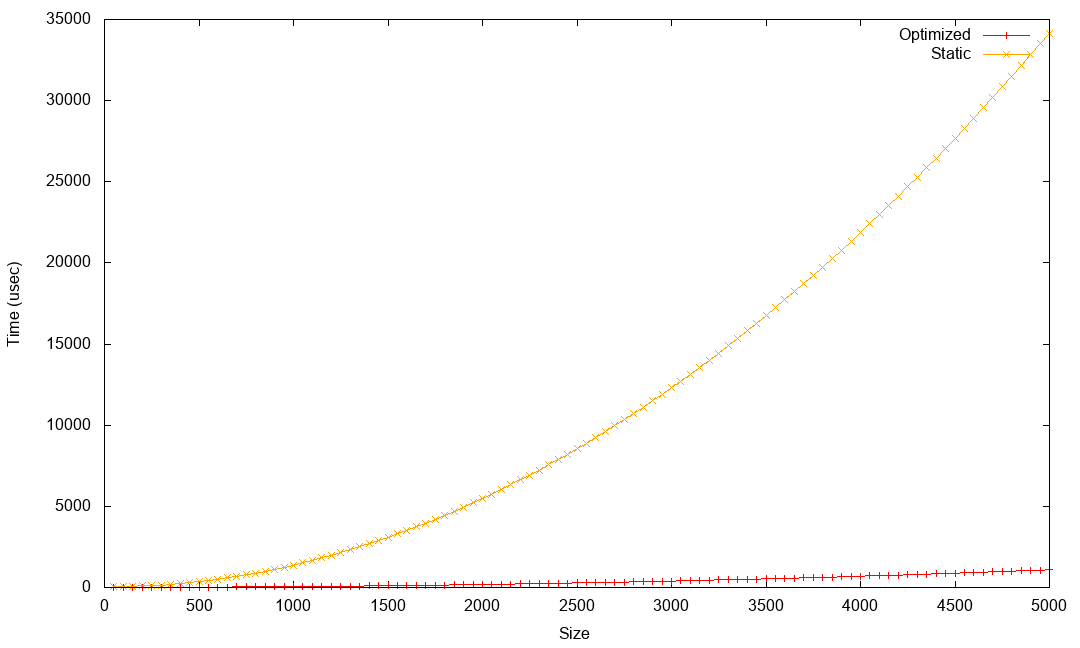
\includegraphics[width=10cm,keepaspectratio]{analysis_grids.png}
	\caption{Vergleich unterschiedlicher Grid-Parameter}
	\label{fig:analysis_grids}
\end{figure}


%
\subsection{Umwandlung ohne Parallelisierung, mit OpenCV und auf der GPU mit CUDA}
%

Um äußere Einflüsse auf die Laufzeitmessungen möglichst klein zu halten, wurden die Messungen 10-mal durchgeführt und die Durchschnittswerte der einzelnen Messwerte pro Implementierung verwendet.\\

Abbildung \ref{fig:analysis} beschreibt die Gesamtlaufzeit der unterschiedlichen Implementierungen. Die Gesamtlaufzeit enthält im Falle von CUDA das Reservieren des GPU-Speichers, das Kopieren der Daten vom Host zum Device, das Kopieren des Ergebnisses vom Device auf den Host, das Freigeben des GPU-Speichers und das Zurücksetzen des Devices. Aus Abbildung \ref{fig:analysis} ist ersichtlich, dass die Gesamtlaufzeit von der CUDA-Implementierung mit ca. 1,1 Sekunden weit über den Laufzeiten der beiden anderen Implementierungen liegt.

\begin{figure}
	\centering
	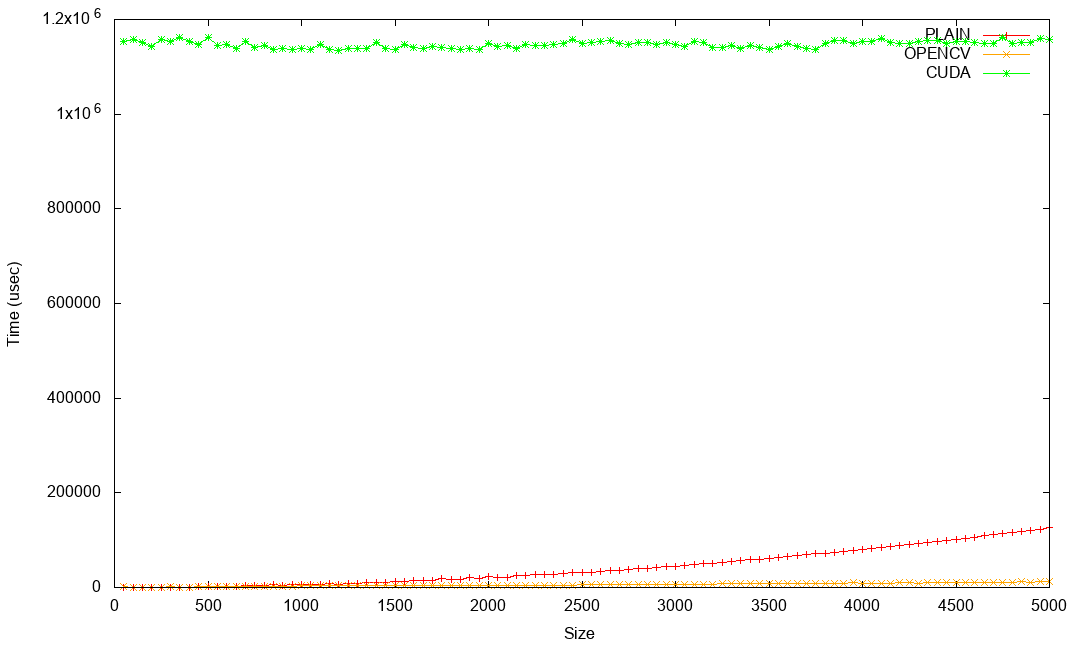
\includegraphics[width=10cm,keepaspectratio]{analysis.png}
	\caption{Gesamtlaufzeit der drei unterschiedlichen Implementierungen}
	\label{fig:analysis}
\end{figure}

Im folgenden ist die OpenCV-Implementierung der Graufstufenkonvertierung dargestellt. Diese Implementierung setzt jedoch im Gegensatz zur CUDA- und CPU-Implementierung voraus, dass das Bild keine Transparenz enthält.

\begin{lstlisting}
result gray(cv::Mat *image, uint32_t width, uint32_t height, uint32_t *data) {
  // This does not work with alpha channel images
  // Only use RGBA images
  transform(*image, *image, Matx13f(0.07, 0.72, 0.21));

  // ...
}
\end{lstlisting}

Um dieses Ergebnis genauer vergleichen zu können, wurde zusätzlich die Laufzeit des Konvertierungsalgorithmus bestimmt. Diese effektiven Laufzeiten unterscheiden sich bei der Implementation ohne Parallelisieren und die Implementierung mit OpenCV nicht von der Gesamtlaufzeit. Bei der CUDA-Implementierung hingegen wird bei der effektiven Laufzeit nur der Aufruf und die Ausführung auf der GPU gemessen. Der Vergleich der effektiven Laufzeit der drei Implementierungen ist in Abbildung \ref{fig:analysis_gpu} dargestellt. Es ist gut zu erkennen, dass die effektive Laufzeit auf der GPU im Vergleich zu den anderen beiden Implementierungen aufgrund der hohen Parallelisierung wesentlich geringer ist.

\begin{figure}
	\centering
	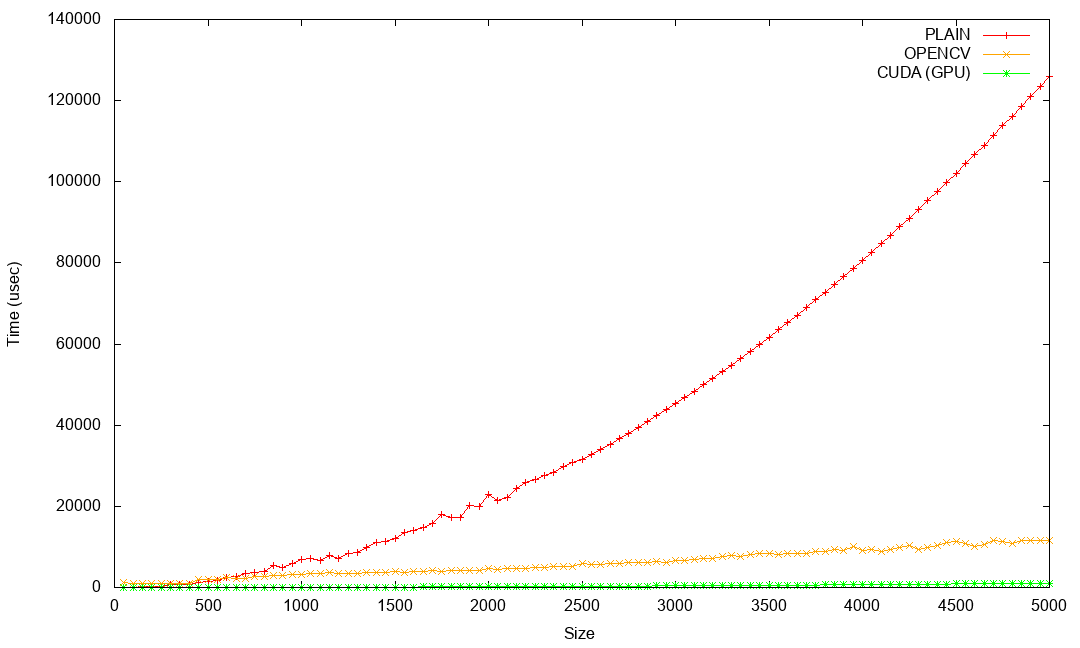
\includegraphics[width=10cm,keepaspectratio]{analysis_gpu.png}
	\caption{Effektive Laufzeit der unterschiedlichen Implementierungen}
	\label{fig:analysis_gpu}
\end{figure}
\newpage
Um einen besseren direkten Vergleich zwischen den Implementierungen mit OpenCV und CUDA zu ermöglichen, ist in Abbildung \ref{fig:analysis_no_plain} der Vergleich zwischen diesen beiden Implementierungen dargestellt. Dabei ist die unterschiedliche Wachstumsgeschwindigkeit deutlich zu erkennen.

\begin{figure}
	\centering
	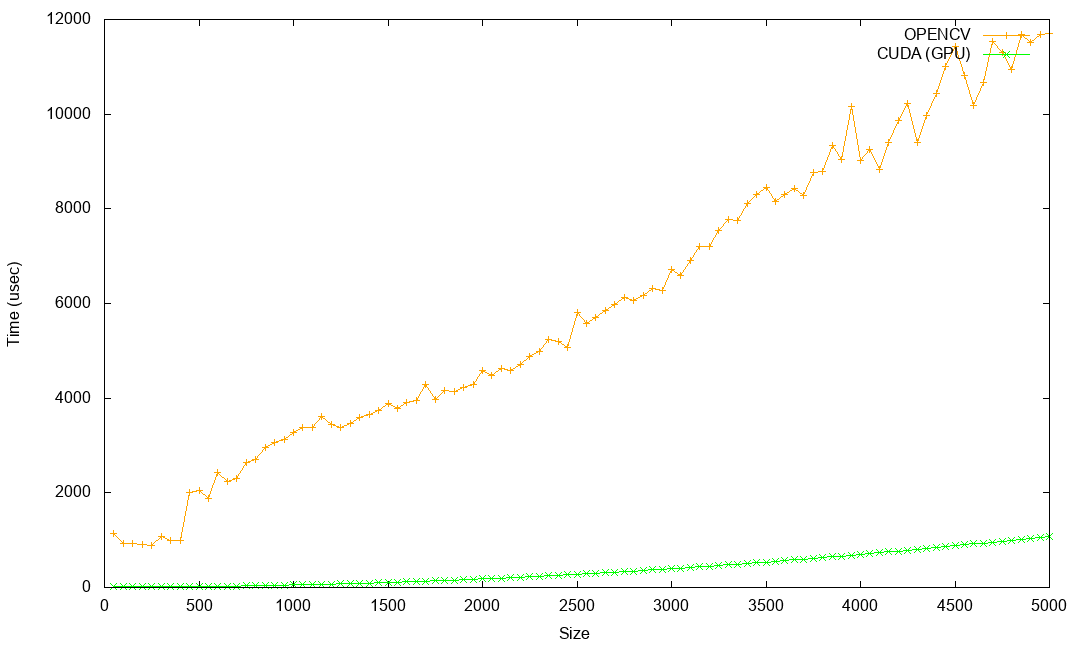
\includegraphics[width=10cm,keepaspectratio]{analysis_no_plain.png}
	\caption{Vergleich der effektiven Laufzeit zwischen CUDA und OpenCV}
	\label{fig:analysis_no_plain}
\end{figure}

%
\section{Fazit}
%

Aus den Performanceuntersuchungen geht hervor, dass der Overhead bei der Verwendung von CUDA nicht zu vernachlässigen ist. Die Verwendung von CUDA eignet sich daher nicht bei kleinen Problemen. Der in der Untersuchung feststellbare Overhead lag bei ca. 1,1 Sekunden. Eine Verwendung eignet sich aufgrund dieser Ergebnisse erst, wenn das zu lösende Problem nicht in weniger als einer Sekunde zu lösen ist.\\

Grundsätzlich ist die Parallelisierung eines Problems ratsam, um die Gesamtlaufzeit möglichst kurz halten.
Es ist von Vorteil, die Auswahl des verwendeten Grids an die Ressourcen des verwendeten Hosts anzupassen. Damit kann eine optimale Ausnutzung der Performance in Bezug auf die Laufzeit erreicht werden.
%
\end{document}
